\section{Causal interventions}
\label{sec:interventions}

\begin{sessioncard}
\textbf{Session 6.} \emph{Goal:} learn the experimental method on which all claims about mechanisms are based:
overwrite one internal value of the model, recompute everything that comes after it, and observe the output.
\emph{Experiments:} where the model stores the information that decides the running example
(\cref{exp:residpatch}), which heads carry this information (\cref{exp:headpatch}), and a fast approximation of
these experiments (\cref{exp:attrpatch}).
\emph{Prerequisites:} sessions 1 to 3.
\end{sessioncard}

Sessions 2 to 5 mostly used observational methods: we recorded activations and found patterns in them. Session
3 showed that such patterns only tell us which information the model \emph{could} use. To learn which information
the model actually uses, we need interventions. Neural networks are unusually well suited for such experiments. We
can set any internal value to any number, recompute the rest of the computation exactly, and repeat this as often
as we
like.

\subsection{Interventions and ablations}

\begin{definition}[Intervention]\label{def:intervention}
A \emph{node} $g$ is any intermediate quantity of the model: the residual stream at one layer and position, the
output of one head, one neuron, one SAE latent. We write $g(\clean)$ for the value of the node when the model
runs on a prompt called $\clean$, and $M(\clean)$ for a number that measures the output on that prompt, called the
\emph{metric}. For a value of the same shape as $g$, the \emph{intervened run} computes everything before the
node as usual, overwrites the node with the given value, and recomputes everything after it. We write
$M(\clean \mid g\leftarrow\text{value})$ for the metric of the intervened run.
\end{definition}

Throughout this session, the metric is the logit difference of the running example. The steering experiments of
session 3 were interventions of this kind. The simplest interventions remove a node. They are called
\emph{ablations}, and they differ in the value that replaces the node.

\begin{center}\small
\begin{tabular}{@{}lp{0.42\textwidth}p{0.38\textwidth}@{}}
\toprule
Ablation & Value written to the node & Main weakness \\
\midrule
zero & $0$ & zero can be far from every value the node normally takes \\
mean & average of the node over a reference set of prompts & the average may be a value that never occurs \\
resample & value of the node on another, randomly chosen prompt & noisy, has to be averaged over many draws \\
\bottomrule
\end{tabular}
\end{center}

\begin{caution}
An ablation compares the model with a modified model, and the replacement value determines the modified model.
Consider a head that always writes roughly the same large vector. Zero ablation removes this constant vector, and
later layers may rely on it for reasons that have nothing to do with the task. Every ablation result should
therefore be reported together with the replacement value that was used.
\end{caution}

\subsection{Activation patching}
\label{sec:patching}

\begin{figure}[t]
\centering
\begin{tikzpicture}[>=Latex, font=\small, n/.style={circle, draw=tutgrey, minimum size=6mm, inner sep=0pt, fill=#1}]
\def\rowa{0} \def\rowb{-1.3} \def\rowc{-2.6}
% clean row
\node[anchor=east] at (2.2,\rowa) {clean prompt};
\foreach \x in {3,4.3,5.6,6.9} {\node[n=tutblue!45] at (\x,\rowa) {};}
\draw[->,tutgrey] (2.3,\rowa) -- (2.68,\rowa);
\foreach \x in {3.32,4.62,5.92} {\draw[->,tutgrey] (\x,\rowa) -- +(0.66,0);}
\draw[->,tutgrey] (7.22,\rowa) -- (7.9,\rowa) node[right, text=black] {$M(\clean)=3.70$};
% patched row
\node[anchor=east, align=right] at (2.2,\rowb) {corrupted prompt,\\ node $g$ patched};
\node[n=tutred!45] at (3,\rowb) {}; \node[n=tutred!45] at (4.3,\rowb) {};
\node[n=tutblue!45, line width=1.2pt] (pg) at (5.6,\rowb) {$g$};
\node[n=tutblue!25!tutred!30] at (6.9,\rowb) {};
\draw[->,tutgrey] (2.3,\rowb) -- (2.68,\rowb);
\draw[->,tutgrey] (3.32,\rowb) -- +(0.66,0);
\draw[->,tutgrey, dashed] (4.62,\rowb) -- +(0.66,0);
\draw[->,tutgrey] (5.92,\rowb) -- +(0.66,0);
\draw[->,tutgrey] (7.22,\rowb) -- (7.9,\rowb) node[right, text=black] {$M(\corr\mid g\leftarrow g(\clean))$};
\draw[->, line width=1.1pt, tutblue] (5.6,-0.32) -- (pg.north);
% corrupted row
\node[anchor=east] at (2.2,\rowc) {corrupted prompt};
\foreach \x in {3,4.3,5.6,6.9} {\node[n=tutred!45] at (\x,\rowc) {};}
\draw[->,tutgrey] (2.3,\rowc) -- (2.68,\rowc);
\foreach \x in {3.32,4.62,5.92} {\draw[->,tutgrey] (\x,\rowc) -- +(0.66,0);}
\draw[->,tutgrey] (7.22,\rowc) -- (7.9,\rowc) node[right, text=black] {$M(\corr)=-4.33$};
\end{tikzpicture}
\caption{Activation patching in the denoising direction. The model runs on the corrupted prompt. One node $g$ is
overwritten with its value from the clean run, and everything after it is recomputed. If the metric moves from
$M(\corr)$ towards $M(\clean)$, the node carries information that distinguishes the two prompts.}
\label{fig:patching-schema}
\end{figure}

\emph{Activation patching} improves on resample ablation by choosing the other prompt deliberately instead of at
random \citep{vig2020investigating,wang2023interpretability}. We prepare two prompts of the same length that differ
only in the aspect that we want to study. In the running example, we use the two prompts
\begin{center}
\begin{tabular}{@{}ll@{}}
$\clean$: & \tok{When Mary and John went to the store, John gave a drink to} \\
$\corr$: & \tok{When Mary and John went to the store, Mary gave a drink to}
\end{tabular}
\end{center}
The corrupted prompt differs from the clean prompt in one token, the second occurrence of the subject. As a
result, the correct continuation of the corrupted prompt is the other name, \tok{John}. For both prompts, the metric
is the logit difference in favour of the name that is correct for the clean prompt, here \tok{Mary}. Averaged over
our 12 pairs of prompts, $M(\clean)=3.70$ and $M(\corr)=-4.33$. So the metrics of the two runs differ by $8.04$
logits. We now run the model on one of the two prompts, and we overwrite a single node with its value from the run
on the other prompt (\cref{fig:patching-schema}). This can be done in two directions.

\begin{definition}[Denoising and noising]\label{def:patching}
The \emph{denoising} effect of a node $g$ is the fraction of the gap that is restored when the corrupted run
receives the clean value of $g$,
\begin{equation}\label{eq:denoise}
\frac{M\big(\corr \mid g\leftarrow g(\clean)\big)-M(\corr)}{M(\clean)-M(\corr)} .
\end{equation}
The \emph{noising} effect of $g$ is the fraction of the gap that is lost when the clean run receives the
corrupted value of $g$,
\begin{equation}\label{eq:noise}
\frac{M(\clean)-M\big(\clean \mid g\leftarrow g(\corr)\big)}{M(\clean)-M(\corr)} .
\end{equation}
\end{definition}
Both numbers are $0$ for a node that plays no role and $1$ for a node that carries the whole difference between
the two prompts.

\begin{experiment}[Where is the information?]\label{exp:residpatch} \script{exp\_ioi.py}
As a first overview, we take as nodes the residual stream $x_i^{(\ell)}$ at every layer $\ell$ and position $i$.
\Cref{fig:residpatch} shows the denoising effect of each of these $12\times15$ nodes. Each part of the figure has a
simple explanation.
\begin{itemize}
\item At all positions before S2, the effect is exactly zero. The two prompts are identical up to S2, and a
position never receives information from later positions. So the two runs have identical streams at these
positions.
\item At S2, the effect is $1.00$ in layers $0$ to $3$. If we restore the stream at the only position where the two
prompts differ, and we do so early enough, we restore the clean run completely. At S2, the effect is still $0.92$ at
the input of layer $7$. It falls to $0.73$ at layer $8$ and to $0.07$ at layer $9$.
\item At the last position, the effect is zero up to layer $6$. It is $0.40$ at the input of layer $8$ and $0.96$ at
the input of layer $9$.
\end{itemize}
So the information about which name is repeated stays at S2 until about layer $7$. Layers $7$ and $8$ then move
it to the last position. Only attention heads can move information between positions (\cref{sec:facts}). The logit
lens of \cref{exp:lens} showed that the answer appears one layer later, in layer 9. Together, the two figures
suggest an order of events. First, the information about the repeated name arrives at the last position. Then, in
layer 9, the name mover heads use this information to write the answer.
\end{experiment}

\begin{figure}[t]
\centering
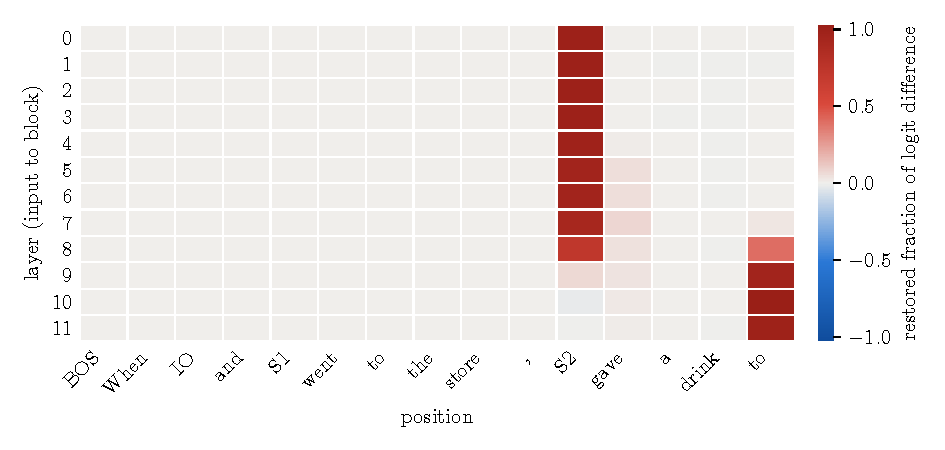
\includegraphics[width=0.86\textwidth]{figures/fig_resid_patching.pdf}
\caption{Activation patching of the residual stream of GPT-2 small on the IOI task (\cref{exp:residpatch}). Each
cell shows the denoising effect \eqref{eq:denoise} of the stream at the input of one layer at one position,
averaged over 12 pairs of prompts.}
\label{fig:residpatch}
\end{figure}

\begin{caution}
The choice of the corrupted prompt determines what a patching experiment can find. Our corrupted prompt changes
which name is repeated, and it keeps everything else the same. Some components are needed for the task but behave
in the same way on both prompts, for example the components that decide that the next token should be a name at
all. These components remain invisible in our experiment. A different question requires a different pair of
prompts \citep{zhang2024towards}.
\end{caution}

\subsection{Sufficient, necessary, direct, total}
\label{sec:necessity}

\begin{experiment}[Patching every head]\label{exp:headpatch} \script{exp\_ioi.py}
We now take the output of each attention head, at all positions, as a node. \Cref{tab:heads} lists four numbers
for twelve heads. The first number is the direct logit attribution of \cref{exp:dla}. The second number is the
denoising effect \eqref{eq:denoise}. The last two numbers describe the noising experiment, in logits. In this
experiment, we replace the output of the head by its output on the corrupted prompt. The \emph{total effect} is the
resulting drop of the metric. The \emph{direct effect} is the part of this drop that comes from the change of the
head's own term in \eqref{eq:dla-ld}, computed with the final scale $\scale(x_n^{(L)})$ of the clean run. The class
names in the table are those of \citet{wang2023interpretability}. Session 7 explains them, and for now they are only
labels.
\end{experiment}

\begin{table}[t]
\centering\small
\begin{tabular}{@{}llrrrr@{}}
\toprule
 & & & denoising & \multicolumn{2}{c}{noising (logits)} \\
\cmidrule(l){5-6}
Head & Class & DLA & effect & direct effect & total effect \\
\midrule
9.9 & name mover & $3.57$ & $0.29$ & $7.00$ & $1.40$ \\
9.6 & name mover & $1.10$ & $0.01$ & $2.27$ & $-0.77$ \\
10.0 & name mover & $0.59$ & $0.09$ & $1.31$ & $0.57$ \\
10.7 & negative name mover & $-2.52$ & $-0.52$ & $-4.62$ & $-3.83$ \\
11.10 & negative name mover & $-1.05$ & $-0.28$ & $-2.24$ & $-2.15$ \\
\addlinespace
8.6 & S-inhibition & $0.00$ & $0.37$ & $0.01$ & $1.55$ \\
8.10 & S-inhibition & $0.44$ & $0.34$ & $0.73$ & $1.51$ \\
7.9 & S-inhibition & $0.19$ & $0.22$ & $0.42$ & $1.17$ \\
7.3 & S-inhibition & $0.22$ & $0.14$ & $0.42$ & $0.96$ \\
\addlinespace
5.5 & induction & $0.00$ & $0.33$ & $0.00$ & $1.46$ \\
6.9 & induction & $0.00$ & $0.15$ & $0.00$ & $0.37$ \\
3.0 & duplicate token & $0.00$ & $0.15$ & $0.00$ & $0.45$ \\
\bottomrule
\end{tabular}
\caption{Four views of twelve attention heads of GPT-2 small on the IOI task (\cref{exp:headpatch}), averaged
over 12 pairs of prompts. DLA is in logits, the denoising effect is a fraction of the gap of $8.04$ logits
between the clean and the corrupted run, and the two noising columns are in logits.}
\label{tab:heads}
\end{table}

The table illustrates three lessons, which hold far beyond this example.

\paragraph{Lesson 1: direct logit attribution misses the early part of a mechanism.} Heads 8.6, 5.5, 6.9 and 3.0
have a DLA of zero. They write nothing in the direction that separates the two names at the output. But corrupting
head 8.6 or head 5.5 alone lowers the metric by about $1.5$ logits. These heads matter because later heads use
their output. Only an intervention can reveal such heads.

\paragraph{Lesson 2: the total effect can be much smaller than the direct effect.} Corrupting the name mover 9.9
removes $7.00$ logits of its direct contribution, but the metric drops by only $1.40$. So the layers after head 9.9
undo four fifths of the damage. For head 9.6, the total effect is even negative: the model does slightly better
when this head, which normally helps, is corrupted. \citet{wang2023interpretability} observed the same effect. They
found heads that take over the job of the name movers when the name movers are removed, and they call these heads
\emph{backup name movers}. \citet{mcgrath2023hydra} studied such compensation systematically. The consequence is
important: if removing a component changes the output only a little, this does not show that the component is
unimportant.

\paragraph{Lesson 3: noising and denoising answer different questions.} Denoising asks whether the clean value
of one node is \emph{sufficient} to move a corrupted run towards the clean behaviour. Noising asks whether the
clean value of one node is \emph{necessary} for the clean behaviour. If several components do the same job in
parallel, each is sufficient and none is necessary. If several components are needed jointly, each is necessary
and none is sufficient (\cref{ex:andor}).

\paragraph{Paths.} Patching a node changes everything that is computed after the node. To find out through which
later components a node acts, we can patch the node only along selected paths. For example, to measure the part of
the effect of head 8.6 that passes through head 9.9, we recompute the input of head 9.9 with the corrupted output of
head 8.6, and we keep the clean output of head 8.6 everywhere else. This method is called \emph{path patching} \citep{wang2023interpretability}.

\subsection{A linear shortcut}
\label{sec:attrpatching}

Patching needs one run of the model for every node. For 144 heads this is cheap. For every neuron at every
position, or for the $24{,}576$ latents of session 5, it is expensive. \emph{Attribution patching}
\citep{nanda2023attribution,syed2024attribution} estimates all patching effects at once. Fix a node $g$, and
consider the metric of the corrupted run as a function of the value written to $g$. A first-order Taylor expansion
of this function around the value $g(\corr)$ gives
\begin{equation}\label{eq:attrpatch}
M\big(\corr \mid g\leftarrow g(\clean)\big)-M(\corr) \;\approx\;
\big(g(\clean)-g(\corr)\big)^\top\,\nabla_gM(\corr),
\end{equation}
where $\nabla_gM(\corr)$ is the gradient of the metric with respect to the node, in the unmodified corrupted run.
To compute the right-hand side for all nodes, we need the values of all nodes on both prompts, which two forward
passes provide, and the gradients with respect to all nodes, which one backward pass provides.

\begin{experiment}[How good is the shortcut?]\label{exp:attrpatch} \script{exp\_ioi.py}
\Cref{fig:attrpatch} compares the estimate \eqref{eq:attrpatch} with the exact denoising effect for all 144
heads. The correlation between the two is $0.98$, and the estimate finds the same important heads. Its largest
errors occur for two heads with large effects. For head 9.9 it gives $0.43$ where the exact value is $0.29$, and for
head 5.5 it gives $0.25$ where the exact value is $0.33$. The estimate is based on a linear approximation, so it is
inaccurate when the metric is far from linear between the two values of the node. In practice, attribution
patching is used as a fast first filter, and the nodes that it selects are then patched exactly.
\end{experiment}

\begin{figure}[t]
\centering
\begin{minipage}[c]{0.42\textwidth}
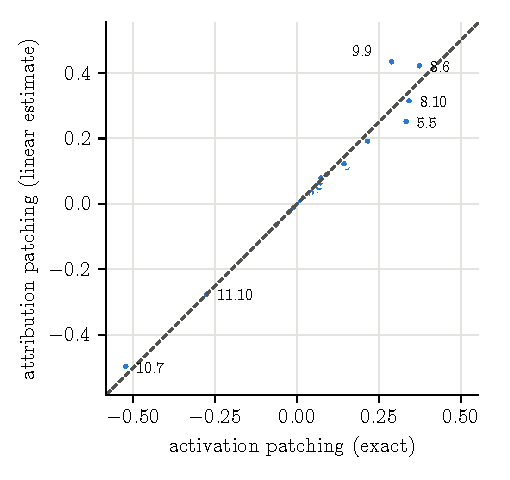
\includegraphics[width=\textwidth]{figures/fig_attr_vs_act.pdf}
\end{minipage}\hfill
\begin{minipage}[c]{0.52\textwidth}
\caption{Attribution patching against activation patching for the 144 attention heads of GPT-2 small on the IOI
task (\cref{exp:attrpatch}). Each dot is one head. The horizontal axis is the exact denoising effect
\eqref{eq:denoise}, and the vertical axis is the linear estimate \eqref{eq:attrpatch} divided by the same gap.}
\label{fig:attrpatch}
\end{minipage}
\end{figure}

\begin{takeaways}
An intervention overwrites a node and recomputes everything after it. The replacement value determines which
question the intervention answers. Activation patching takes the replacement value from a minimally different
prompt, and it finds where the model stores the information that distinguishes the two prompts. In the running
example, this information moves from the repeated name to the last position in layers 7 and 8. Direct effects,
total effects, sufficiency and necessity are four different things, and compensation by later layers can hide
important components.
\end{takeaways}

\subsection*{Questions for the seminar}

\begin{exercise}[Sufficient or necessary]\label{ex:andor}
A model has two binary nodes $g_1,g_2$. On the clean prompt both are $1$, on the corrupted prompt both are $0$.
Compute the denoising effect \eqref{eq:denoise} and the noising effect \eqref{eq:noise} of $g_1$ when the metric
is (a) $M=\max(g_1,g_2)$ and (b) $M=\min(g_1,g_2)$. Relate the result to Lesson 3.
\end{exercise}

\begin{exercise}[Mean ablation and resampling]\label{ex:meanresample}
Let $g$ be a node with real values. (a) Show that if the metric of the intervened run is an affine function of
the value written to $g$, then the metric under mean ablation equals the average, over the reference prompts, of
the metric under resample ablation. (b) Let $g$ take the value $+1$ on one half of the reference prompts and
$-1$ on the other half, and let the metric of the intervened run be the square of the value written to $g$.
Compute the metric under both ablations. (c) Which of the two results describes a state that the model can
actually be in?
\end{exercise}

\begin{exercise}[Designing a patching experiment]\label{ex:design}
We want to find out where a model stores and uses the fact that the Eiffel Tower is in Paris, with the prompt
\tok{The Eiffel Tower is located in the city of}. (a) Propose a corrupted prompt and a metric. (b) Which
components can the experiment find, and which components that the task needs will it miss? (c) Use
\cref{tab:predictions} to say why GPT-2 small is the wrong model for this experiment.
\end{exercise}

\begin{exercise}[The error of the linear estimate]\label{ex:trapezoid}
Let $g$ be a node with real values, and suppose that the metric of the corrupted run, as a function of the value
written to $g$, is the square of that value. Let $g(\corr)=1$ and $g(\clean)=3$. (a) Compute the exact patching
effect and the estimate \eqref{eq:attrpatch}. (b) Replace the gradient in \eqref{eq:attrpatch} by the average of
the gradients at the two values, and show that the estimate becomes exact. (c) Why is the estimate of (b) exact
for every polynomial of degree two?
\end{exercise}

\begin{readinglist}
\item \citet{vig2020investigating}, \emph{NeurIPS}. Brings causal mediation analysis to language models, and with
it the vocabulary of direct and indirect effects.
\item \citet{meng2022locating}, \emph{NeurIPS}, and \citet{hase2023does}, \emph{NeurIPS}. Localisation of facts by
patching, and the later finding that the localisation does not predict where editing a fact works.
\item \citet{zhang2024towards}, \emph{ICLR}. A systematic study of how the choice of corruption and of metric
changes the conclusions of a patching experiment.
\item \citet{rushing2024explorations}, \emph{ICML}. Measures the compensation of Lesson 2 over a whole data set
and identifies two mechanisms behind it.
\end{readinglist}
